%(BEGIN_QUESTION)
% Copyright 2006, Tony R. Kuphaldt, released under the Creative Commons Attribution License (v 1.0)
% This means you may do almost anything with this work of mine, so long as you give me proper credit

Anta at en liten gummiball flyter i fluidet inne i en hydraulikksylinder som vist under. Hva skjer med ballen når en skyvekraft påføres sylinderstangen? Hva skjer med ballen når en trekkraft påføres stangen?

$$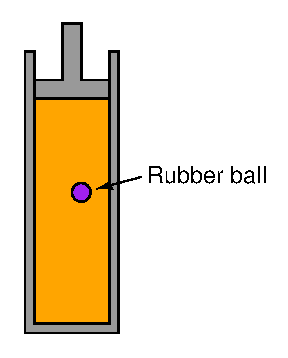
\includegraphics[height=9cm]{i00143x01.eps}$$

\underbar{file i00143}
%(END_QUESTION)





%(BEGIN_ANSWER)

En skyvekraft på stangen vil komprimere gummiballen til mindre diameter. En trekkraft vil utvide ballen til større diameter.

$$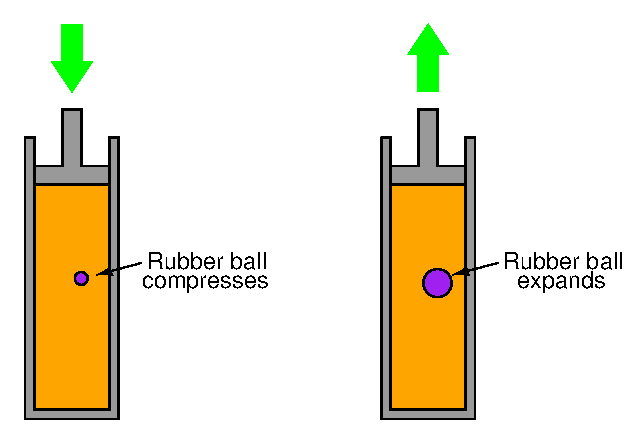
\includegraphics[width=15.5cm]{i00143x02.eps}$$

%(END_ANSWER)





%(BEGIN_NOTES)

En skyvekraft på stangen komprimerer gummiballen, fordi fluidtrykket virker i alle retninger, inkludert inn mot ballens sentrum. En trekkraft vil utvide ballen fordi vakuumet (negativt trykk) som dannes vil {\it trekke} i alle retninger.

$$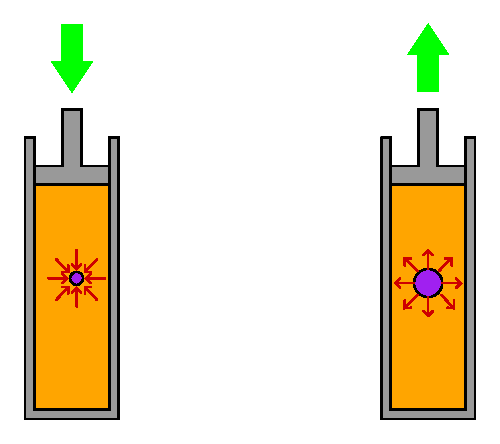
\includegraphics[width=15.5cm]{i00143x03.eps}$$

%INDEX% Physics, static fluids: direction of force exerted by fluid pressure

%(END_NOTES)
